\documentclass[hyperref]{article}
%MS%%%%%%%%%%%%%%%%%%%% Article Format %%%%%%%%%%%%%%%%%
%+++++++++++++++++++++ Usepackage +++++++++++++++%%
\usepackage{graphicx} %% Package for Figure
\usepackage{float} %% Package for Float
\usepackage{amssymb}
\usepackage{amsmath}
\usepackage{mathtools}
\usepackage[thmmarks,amsmath]{ntheorem} %% If amsmath is applied, then amsma is necessary
\usepackage{bm} %% Bold Mathematical Symbols
\usepackage[colorlinks,linkcolor=cyan,citecolor=cyan]{hyperref}
\usepackage{extarrows}
\usepackage[hang,flushmargin]{footmisc} %% Let the footnote not indentation
\usepackage[square,comma,sort&compress,numbers]{natbib} %% Sort of References
\usepackage{mathrsfs} %% Swash letter
\usepackage[font=footnotesize,skip=0pt,textfont=rm,labelfont=rm]{caption,subcaption} 
%% Format of Caption for Tab. and Fig.
\usepackage{booktabs} %% tables with three lines
\usepackage{tocloft}
\usepackage{graphicx}
\usepackage{algorithm}
\usepackage{algorithmic}

%+++++++++++++++ Proof etc. +++++++++++++++++++++++++%%
{%% Environment of Proof
	\theoremstyle{nonumberplain}
	\theoremheaderfont{\bfseries}
	\theorembodyfont{\normalfont}
	\theoremsymbol{\mbox{$\Box$}}
	\newtheorem{proof}{Proof}
}

\usepackage{theorem}
\newtheorem{theorem}{Theorem}[section]
\newtheorem{lemma}{Lemma}[section]
\newtheorem{definition}{Definition}[section]
\newtheorem{assumption}{Assumption}[section]
\newtheorem{example}{Example}[section]
\newtheorem{corollary}{Corollary}[section]
{%% Environment of Remark
	\theoremheaderfont{\bfseries}
	\theorembodyfont{\normalfont}
	\newtheorem{remark}{Remark}[section]
}
\usepackage{abstract}
\renewcommand{\abstractnamefont}{\Large\bfseries}
%\numberwithin{equation}{section} %% Number of Equation
%++++++++++++++++++++++++++++++++ Page format ++++++++++++++++++++++++++%%
\graphicspath{{figure/}}                                 %% Path of Figures
\usepackage[a4paper]{geometry}                           %% Paper size
\geometry{left=2.5cm,right=2.5cm,top=2.5cm,bottom=2.5cm} %% Margin
\linespread{1.2}      

% matlab code package
\usepackage{appendix}
\usepackage{listings}%插入代码
\usepackage{color}
\lstset{%代码格式的配置
	extendedchars=false,            % Shutdown no-ASCII compatible
	language=Matlab,                % !!!选择代码的语言
	basicstyle=\footnotesize\tt,    % the size of the fonts that are used for the code
	tabsize=3,                            % sets default tabsize to 3 spaces
	numbers=left,                   % where to put the line-numbers
	numberstyle=\tiny,              % the size of the fonts that are used for the line-numbers
	stepnumber=1,                   % the step between two line-numbers. If it's 1 each line
	% will be numbered
	numbersep=5pt,                  % how far the line-numbers are from the code   %
	keywordstyle=\color[rgb]{0,0,1},                % keywords
	commentstyle=\color[rgb]{0.133,0.545,0.133},    % comments
	stringstyle=\color[rgb]{0.627,0.126,0.941},      % strings
	backgroundcolor=\color{white}, % choose the background color. You must add \usepackage{color}
	showspaces=false,               % show spaces adding particular underscores
	showstringspaces=false,         % underline spaces within strings
	showtabs=false,                 % show tabs within strings adding particular underscores
	frame=single,                   % adds a frame around the code
	captionpos=b,                   % sets the caption-position to bottom
	breaklines=true,                % sets automatic line breaking
	breakatwhitespace=false,        % sets if automatic breaks should only happen at whitespace
	title=\lstname,                 % show the filename of files included with \lstinputlisting;
	% also try caption instead of title
	mathescape=true,escapechar=?    % escape to latex with ?..?
	escapeinside={\%*}{*)},         % if you want to add a comment within your code
	%columns=fixed,                  % nice spacing
	%morestring=[m]',                % strings
	%morekeywords={%,...},%          % if you want to add more keywords to the set
	%    break,case,catch,continue,elseif,else,end,for,function,global,%
	%    if,otherwise,persistent,return,switch,try,while,...},%
}
%\usepackage{subfigure}

                                   %% Line Spread
%MS%%%%%%%%%%%%%%%%%%%%%%%%%%%% End Format %%%%%%%%%%%%%%%%%%%%%%%%%%%%%%%%%%

%MS%%%%%%%%%%%%%%%%%%%%%%%%%%%%%%%%%%%%%%%%%%%
%MS                                         %%
%MS        The Main Body begins here        %%
%MS                                         %%
%MS%%%%%%%%%%%%%%%%%%%%%%%%%%%%%%%%%%%%%%%%%%%

%MS++++++++++++++++++++++++++++++ Title +++++++++++++++++++
\title{Machine Vision Computing Project}
\author{\textup{Chen Yihui \ A0263115N\\
				Yang Jiaqi \ \ A\\
			    Yang Yitian  A}}
\begin{document}
	\begin{titlepage}
		\center
		\newcommand{\HRule}{\rule{\linewidth}{0.5mm}}
		
\includegraphics[width=8cm]{logo.png}\\[1cm] 
		\quad\\[1.5cm]
		\textsl{\Large National University of Singapore}\\[0.5cm] 
		\textsl{\large College of Design and Engineering}\\[0.5cm]
		\makeatletter
		\HRule \\[0.4cm]
		{ \huge \bfseries \@title}\\[0.4cm] 
		\HRule \\[1.5cm]
		\begin{minipage}{0.4\textwidth}
			\begin{flushleft} \large
				\emph{Authors:}\\
				\@author 
			\end{flushleft}
		\end{minipage}
		~
		\begin{minipage}{0.4\textwidth}
			\begin{flushright} \large
				\emph{Supervisor:} \\
				\textup{Prof. Chui Chee Kong\\
						Prof. Guillaume Adrien Sartoretti}
			\end{flushright}
		\end{minipage}\\[3cm]
		\makeatother
		{\Large Assignment for ME5405 Machine Vision}\\[0.5cm]
%		{\large \emph{Matriculation Number: A0263115N}}\\[0.5cm]
%		{\large \emph{Email Address: e1010473@u.nus.edu}}\\[0.5cm]
		{\large \today}\\[2cm] 
		\vfill 
	\end{titlepage}
	

	%MS+++++++++++++++++++++ Abstract +++++++++++++++++++++++++
	\begin{abstract}

	
	
	\end{abstract}
	
	\vspace{1ex}
	{\noindent\small{\bf Keywords:}
		}
	
	\newpage
	
	\tableofcontents
	\newpage
	
	%MS++++++++++++++++++++++++++++++ Main body ++++++++++++++++++++
	\section{Problem statement}

	
	\hspace{1.0em}
	
	In this mini-project, two images are going to be processed. The first image (Fig.~\ref{fig1a}) is a 64x64 32-level image, which is a coded array composed of alphanumeric characters. The range of them is 0-9 and A-V, which corresponds to 32 gray levels. Image 2 (Fig.~\ref{fig1b}) is a JEPG color image with three lines of characters. The main tasks to complete are listed as follows.
	
	\begin{figure}[htbp]
		\centering
		\begin{minipage}[t]{0.48\textwidth}
			\centering
			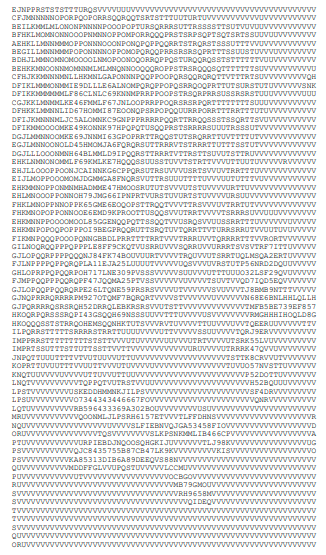
\includegraphics[width=6cm]{fig1.png}
			\subcaption{Image 1}
			\label{fig1a}
		\end{minipage}
		\begin{minipage}[t]{0.48\textwidth}
			\centering
			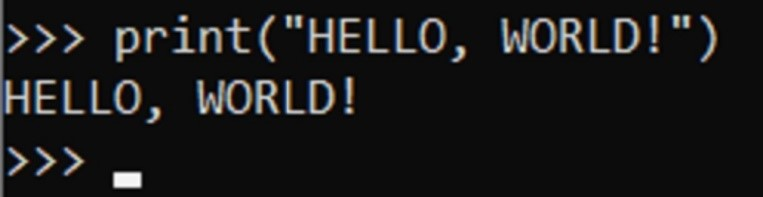
\includegraphics[width=6cm]{fig2.png}
			\subcaption{Image 2}
			\label{fig1b}
		\end{minipage}
		\caption{Task images}
	\end{figure}
	
	\begin{itemize}
		\item Display the two original images on the screen and especially extract the middle line of image 2.
		\item Convert the two images into binary images using different thresholding methods.
		\item Determine a one-pixel thin image for both two images.
		\item Edge detection to determine the outlines of the characters of the both images. 
		\item Label different objects for both images, and also sperate image 2 into characters.
		\item Rotate the original version of image 1 by 30, 60, and 90 degrees respectively.
		\item Train a classifier using machine learning techniques and test the recognition accuracy on sperated characters in image 2.
		\item Experiment with pre-processing of the data and discuss the sensitive of the methods in last step.
		
	\end{itemize}
	
	 Since most of tasks for the two images are similar, we will test various methods for each task and make essential comparisons. In each step, the method with best performance is chosen and the result will be used for further processing. 
	 
	 
	\section{Display the original image and preprocessing}
	
	\hspace{1.0em}
	Since image 1 is composed of numbers and characters, a decoder is need to generate corresponding gray levels. $0-9$ and $A-V$ can be seen as 32 gray levels and the decoded result is shown in Fig.~\ref{fig2a}. As for image 2, we need to convert the 3-channel RGB color image to an 1-channel image with 256 gray levels, and the result is illustrated in Fig.~\ref{fig2b}.
	
	\begin{figure}[htbp]
		\centering
		\begin{minipage}[t]{0.48\textwidth}
			\centering
			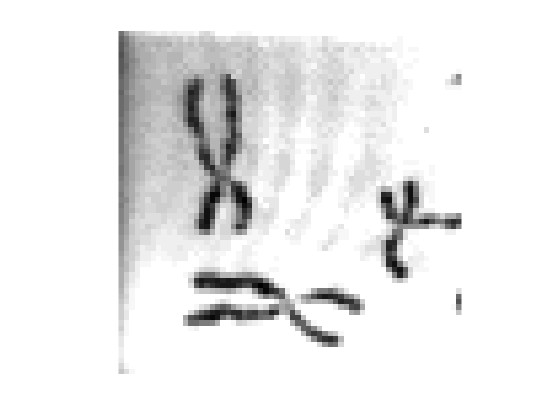
\includegraphics[width=6cm]{fig2a.jpg}
			\subcaption{Image 1}
			\label{fig2a}
		\end{minipage}
		\begin{minipage}[t]{0.48\textwidth}
			\centering
			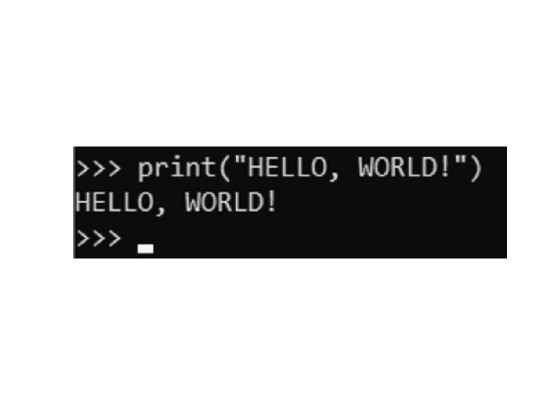
\includegraphics[width=6cm]{fig2b.jpg}
			\subcaption{Image 2}
			\label{fig2b}
		\end{minipage}
		\caption{Original images}
	\end{figure}

	In order to achieve better performance for later tasks, both of the two images should be preprocessed. For image 1, a gaussian filter is applied to smooth the image. On the other side, image 2 contains too much useless information, so the middle line with words "HELLO,WORLD!" is extracted.
	
	The images after preprocessing are shown in Fig.~\ref{fig3}.
	
	\begin{figure}[htbp]
		\centering
		\begin{minipage}[t]{0.48\textwidth}
			\centering
			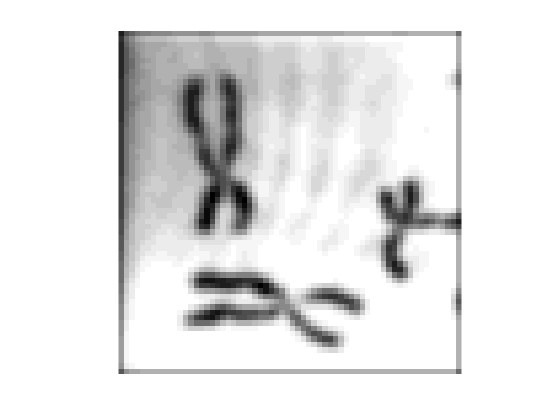
\includegraphics[width=6cm]{fig3a.jpg}
			\subcaption{Image 1}
		\end{minipage}
		\begin{minipage}[t]{0.48\textwidth}
			\centering
			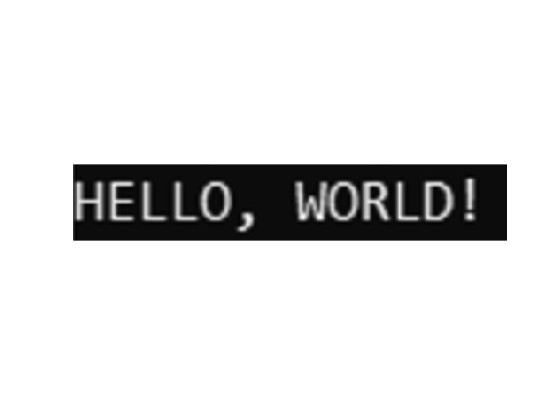
\includegraphics[width=6cm]{fig3b.jpg}
			\subcaption{Image 2}
		\end{minipage}
		\caption{Images after preprocessing}
		\label{fig3}
	\end{figure}
	
	
	
	\section{Binarizing image with thresholding methods}
	
	\hspace{1.0em}
	A raw image usually contains the target object, the background and the noise. When processing images, we need to extract the target object that we are interested and eliminate the noise or useless background pixels. This procedure is called binarizing and has been widely used in image processing. Binary images have only two gray levels that represent black and white respectively. The two gray levels are often set as 0 and 255, or logical value 0 and 1. Therefore, they have small data volume, fast processing speed, low cost and high practicality, and also make it more convenient to define various concepts of geometry. Binary image is generally associated with specific algorithms, many of which require binary data as input.
	
	A common method is to set a threshold $T$ to divide the image pixels into two parts. With this thresholding method, we could convert the original image to binary one and sperate the object from the background. Then the difficulty lies in the choice of thresholding methods, which should be robust given different environment conditions and input images. Moreover, thresholds can be more than one to realize both global and local binarization. Global binarization, like those reliant on histograms, use information from the whole image to find one threshold which will make a binary image. Local binarization determines a different threshold value for every pixel based on characteristics of their surrounding area. Localized techniques are sometimes seen as a panacea for images with small details. 
	
	In this section, we apply six methods that includes both global and local thresholding techniques. We also compare the different performance between them and select the best method fit for later tasks.
	
	\subsection{Mannually threshold setting}
	
	\hspace{1.0em}
	It is easy to think out the idea to simply give a global threshold. Here we mannually test different thresholds around the average gray level intensity of the whole image, and set the threshold as 18 for image 1 while 100 for image 2. It is the simplest method but obviously setting threshold for every image mannually is impossible, and the binarizing performance for different input images will be bad if the global threshold always remains unchanged.
	
%	\subsection{Global mean threshold}
%	
%	\hspace{1.0em}
%	Compared with the former naive method, global mean threshold method solves the applicability problem by using the mean value of all pixels. The mean value of all pixels is calculated and taken as the global threshold. After that, the pixel values which are larger than the global threshold are all set to 1, while the rest are set to 0. The disadvantage is that some object pixels or background pixels may be lost.
	
	\subsection{Iterative method}
	
	\hspace{1.0em}
	The main idea for iterative method is that the sum of two mean values for part A (the gray value higher than threshold) and B (the gray value lower than threshold) after image segmentation remains basically stable. Therefore, as the iteration proceeds, the final convergence value $\frac{mean(A)+mean(B)}{2}$ can be taken as the segmentation threshold. The flow chart for this iterative method is given in Fig.~\ref{fig4}.
	
	\begin{figure}[htbp]
		\centering
			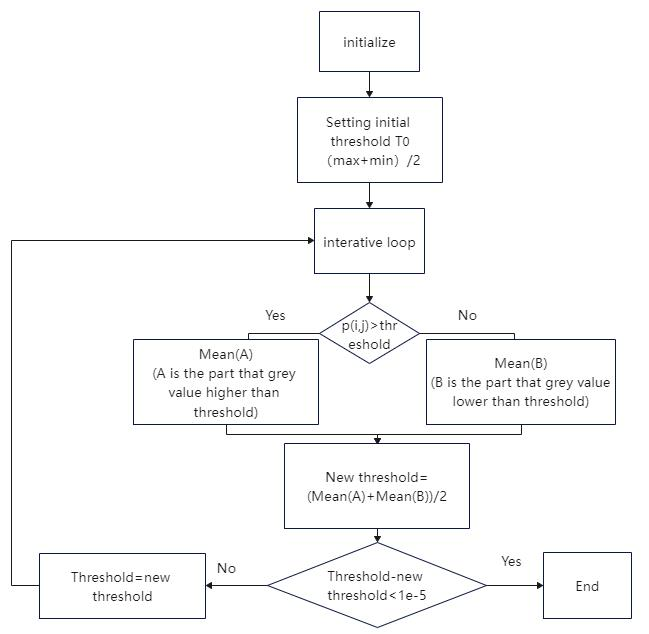
\includegraphics[width=10cm]{fig4.jpg}
			\caption{Flow chart for iterative method}
		\label{fig4}
	\end{figure}
	
	\subsection{OTSU}
	
	\hspace{1.0em}
	OTSU method is an image grayscale adaptive thresholding algorithm, which was proposed by Japanese scholar Otsu in 1979 and thus named by his name. The OTSU method divides the image into two parts according to the distribution of gray values on the image, and the foreground is the part that we are interested in. In the procedure, the intra-class variance between the background and foreground is calculated by iterating through different thresholds. When the intra-class variance achieves the maximum value, the corresponding threshold is the estimed boundary.
	
	According to the OTSU method, we assume the threshold $T_{h}$ could divide the pixels into two parts: $C_{1}$ (higher than $T_{h}$) and $C_{2}$ (lower than $T_{h}$). Suppose that the mean values of the two parts are $m_{1}$ and $m_{2}$, the global mean value of the image is $m_{G}$, and the probability of a pixel being classified into $C_{1}$ and $C_{2}$ classes is $p_{1}$ and $p_{2}$ respectively. Then they satisfy the following equation:
	
	\begin{equation}
	\begin{split}
	\begin{aligned}
	p_{1}m_{1}+p_{2}m_{2}&=m_{G}\\
	p_{1}+p_{2}&=1
	\end{aligned}
	\end{split}
	\label{eq1}
	\end{equation}
	
	According to the concept of variance, the intra-class variance can be written and simplified as:
	
	\begin{equation}
	\begin{split}
	\begin{aligned}
	\sigma ^{2}&=p_{1}(m_{1}-m_{G})^{2}+p_{2}(m_{2}-m_{G})^{2}\\
	&=p_{1}p_{2}(m_{1}-m_{2})^{2}
	\end{aligned}
	\end{split}
	\label{eq2}
	\end{equation}
	
	Because that $p_{1}=\sum_{i=0}^{k}p_{i}$, we get:
	
	\begin{equation}
	\begin{split}
	\begin{aligned}
	m_{1}=\frac{1}{p_{1}}\cdot \sum_{i=0}^{k}ip_{i}, \ \
	m_{2}=\frac{1}{p_{2}}\cdot \sum_{i=K+1}^{L-1}ip_{i}
	\end{aligned}
	\end{split}
	\label{eq3}
	\end{equation}
	
	where $K$ is the evaluated gray level in this iteration, and $L$ is the total gray levels. Then the cumulative mean value $m$ of the gray level $K$ and the global mean value $m_{G}$ of the image are:
	
	\begin{equation}
	\begin{split}
	\begin{aligned}
	m=\sum_{i=0}^{k}ip_{i}&, \ \ m_{G}=\sum_{i=0}^{L-1}ip_{i}\\
	m_{1}=\frac{1}{p_{1}}m&, \ \ m_{2}=\frac{1}{p_{2}}(m_{G}-m)
	\end{aligned}
	\end{split}
	\label{eq4}
	\end{equation}
	
	Combine the expression in Eq.~\ref{eq4} and Eq.~\ref{eq2}, we finally get the intra-class variance:
	
	\begin{equation}
	\begin{split}
	\begin{aligned}
	\sigma ^{2}=\frac{(m_{G}p_{1}-m)^{2}}{p_{1}(1-p_{1})}
	\end{aligned}
	\end{split}
	\label{eq5}
	\end{equation}
	
	The gray level $k$ that maximizes the above expression is the OTSU threshold. Since the variance is a measure of the uniformity of gray distribution, the larger the interclass variance between the background and foreground, the greater the difference between the two parts of the image, and the smaller the difference between the two parts will be when part of the foreground is mis-segmented into the background or part of the background is mis-segmented into the foreground. Therefore, the segmentation with the largest interclass variance implies the smallest probability of misclassification.
	
	OTSU is considered as the best algorithm in image binarization because it is simple to compute and independent of image brightness and contrast so it has been widely used in digital image processing. However, it also has certain disadvantages including the sensitivity to image noise and only available for single target. Moreover, it may loss efficacy when the target and background size ratio is disparate, and the inter-class variance function may present double or multiple peaks at this time.
	
	\subsection{Niblack}
	
	\hspace{1.0em}
	The Niblack algorithm is to calculates a threshold for a pixel based on the points in the neighborhood centered on the pixel point. The threshold for each pixel is calculated by Eq.~\ref{eq6}.
	
	\begin{equation}
	\begin{split}
	\begin{aligned}
	T_{Niblack}=m+ks
	\end{aligned}
	\end{split}
	\label{eq6}
	\end{equation}
	
	In the expression, $m$ is the mean value and $s$ is the standard deviation in the kernel. We use the convolution method, which convolves the image matrix with the all-1 matrix, which is actually the sum of the pixels within this window again. This is more than 10 times faster than traversing pixel by pixel.
	
	The drawback of the Niblack algorithm is that on the one hand, the kernel size will lead to the inability to find the threshold value within the $\frac{r-1}{2}$ pixels in the boundary region. On the other hand, if the $r \times r$ kernel is all background, then the algorithm will inevitably make some of the pixel points become foreground and form pseudo-noise. Therefore, the choice of kernel size is very critical. If the kernel is too small, the noise cannot be effectively suppressed, on the other side it will lead to loss of details.
	
	\subsection{Bernsen}
	
	\hspace{1.0em}
	The main idea of Bernsen is using the maximum and the minimum value from the kernel area of a pixel to set the threshold. Let the current pixel be the point $P(i,j)$, calculate the maximum value $p_{max}$ and the minimum value $p_{min}$ of all pixels in the window of size $k\times k$ centered on $P$. If the value of difference is similar, the part belongs to the target or the background. Then we compare the grayscale with the global threshold to determine whether it is the target or the background, if the difference between the two is larger, it may belong to the edge of the intersection of the target and the background, then the average of the two as the kernel threshold. 
	
	\subsection{Kittler}
	
	\hspace{1.0em}
	The main idea for Kittler method is to calculate the average value of the gradient grayscale of the whole image and use this average value as a threshold. The Kittler algorithm is close to the OTSU method in effect, but is faster (depending on the application scenario) when applied in images with high pixel quality.
	
	According to the definition of partial differentiation of a two-dimensional function, the partial derivatives in the x, y direction can be expressed as:
	
	\begin{equation}
	\begin{split}
	\begin{aligned}
	\frac{\partial f(x,y)}{\partial x}&=\lim_{\varepsilon \rightarrow 0}\frac{f(x+\varepsilon,y)-f(x,y)}{\varepsilon}\\
	\frac{\partial f(x,y)}{\partial y}&=\lim_{\varepsilon \rightarrow 0}\frac{f(x,y+\varepsilon)-f(x,y)}{\varepsilon}
	\end{aligned}
	\end{split}
	\label{eq7}
	\end{equation}
	
	The image is a discrete two-dimensional function, $\varepsilon$ cannot be infinitely small, and our image is discretized by pixel, and the smallest $\varepsilon$ is 0 pixels. Therefore, the image discretization above becomes again of the following form ($\varepsilon=1$).
	
	\begin{equation}
	\begin{split}
	\begin{aligned}
	\frac{\partial f(x,y)}{\partial x}&=f(x+1,y)-f(x,y)=gx\\
	\frac{\partial f(x,y)}{\partial y}&=f(x,y+1)-f(x,y)=gy
	\end{aligned}
	\end{split}
	\label{eq8}
	\end{equation}
	
	This is the gradient of the image in the x-direction and y-direction at the point respectively. From the above expression, it can be seen that the gradient of the image is equivalent to the difference between 2 adjacent pixels. The gradient could be calculated by:
	
	\begin{equation}
	\begin{split}
	\begin{aligned}
	M(x,y)=\sqrt{(gx)^{2}+(gx)^{2}}
	\end{aligned}
	\end{split}
	\label{eq9}
	\end{equation}
	
	By using the Eq.~\ref{eq9} to calculate the gradient, the threshold is the average value of the gradient.
	
	\subsection{Comparison and discussion}
	
	\hspace{1.0em}
	The algorithm we applied above include both global binarization and local binarization techniques, the feature of which have been given in the beginning of this part. So we can analyze that mannual set method, iterative method, OTSU and Kittler algorithm are global binarization while Bernsen and Niblack are local binarization.  
	
	The mannually set is the simplest but they could be affected by changes in image contrast and brightness and other factor so the effects are not excellent. The iterative method has well performance when distinguishing the foreground and background of the image. However, it can’t distinguish the fine points of the image sometimes, and the time complexity of the algorithm is relatively high. As for OTSU, for images with different brightness conditions, as long as the brightness is uniform, the processing effect is better and the algorithm is more stable with low time complexity. We can also find from the comparation between different algorithm when handling the image 1 in Fig.~\ref{fig5}, the effect of OTSU is excellent. Kittler algorithm has a similar effect to the OTSU in many scenarios but it is susceptible to noise so maybe it is not quite suitable for our image.
	
	\begin{figure}[htbp]
		\centering
			\centering
			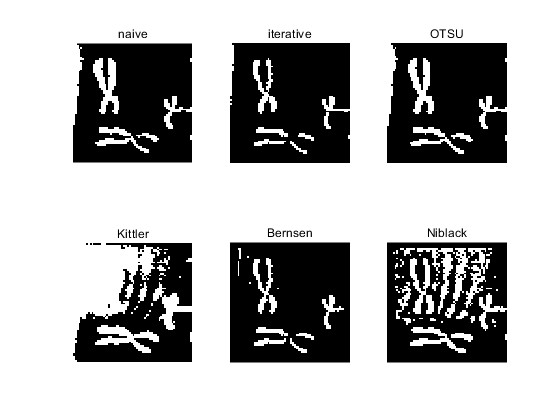
\includegraphics[width=10cm]{fig5.jpg}
		\caption{The performance of different binarizing algorithms for image 1}
		\label{fig5}
	\end{figure}
	
	The advantage of local binarization is that it could process the image with uneven illumination better. For example if we want to deal with Fig.~\ref{fig6}, when the global threshold is performed directly, the upper left half of the sushi is revealed while the lower right half is still black. The problem of global binarization is that no matter what threshold parameters are set, the full map requirement cannot be met.
	
	\begin{figure}[htbp]
		\centering
		\centering
		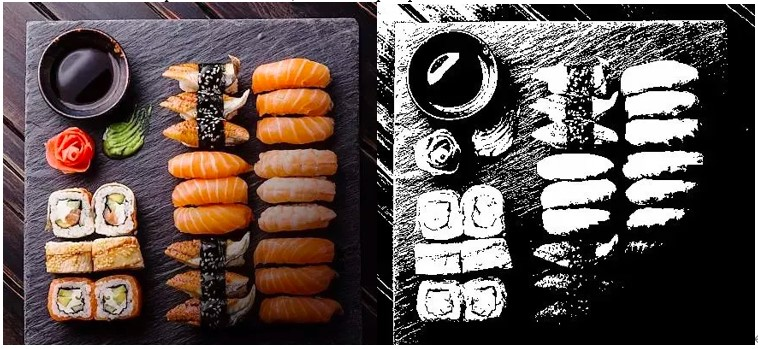
\includegraphics[width=10cm]{fig6.jpg}
		\caption{Example to introduce the disadvantage of global binarization}
		\label{fig6}
	\end{figure}

	By using the local binarization we could solve the problem above. However, the effect of the algorithm has a large relationship with the select of windows or kernel size, the choice of kernel size is very critical. So it may take long time to select a proper parameter. As shown in Fig.~\ref{fig5}, the OTSU algorithm already has quite excellent performance and it is more stable with low time complexity. The image also does not have obviously uneven illumination problem, so we choose OTSU algorithm to binarize image 1.
	
	As for image 2, the performance of different algorithms are shown in Fig.~\ref{fig7}, where OTSU algorithm also shows the best result.
	
	\begin{figure}[h]
		\centering
		\centering
		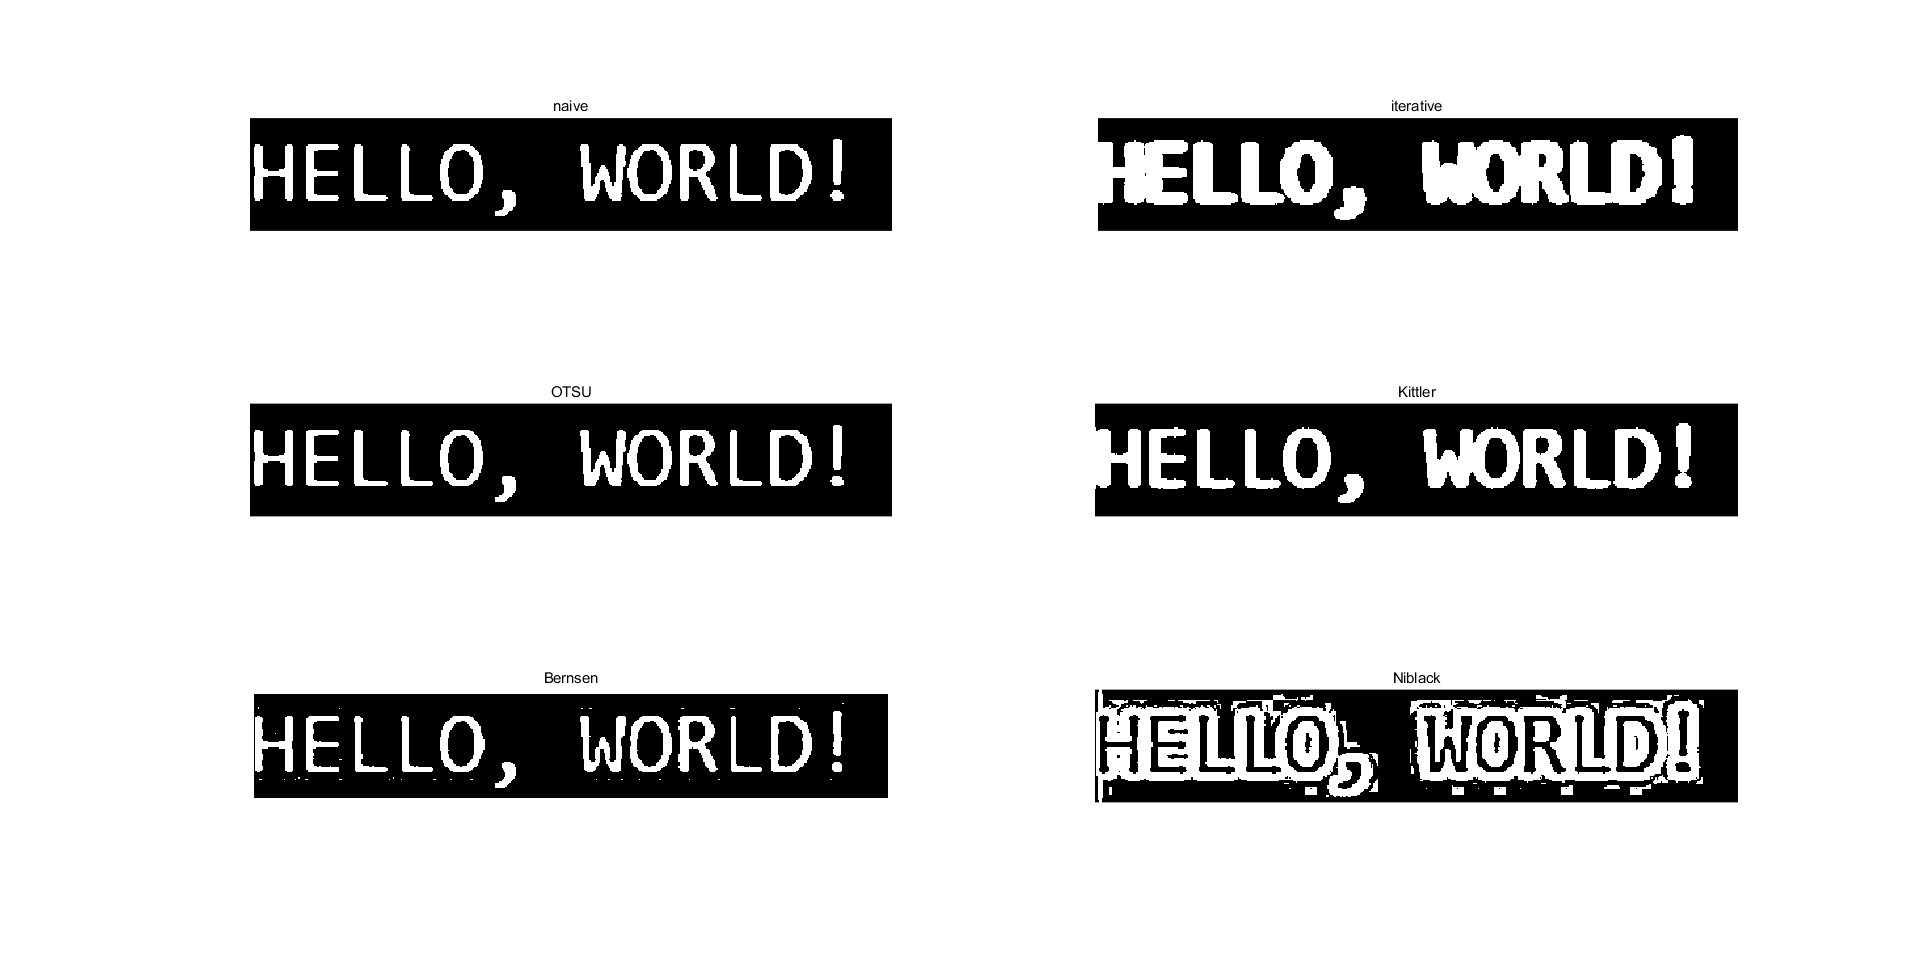
\includegraphics[width=12cm]{fig7.jpg}
		\caption{The performance of different binarizing algorithms for image 2}
		\label{fig7}
	\end{figure}
	
	
	
	\subsection{Chosen algorithm}
	
	\hspace{1.0em}
	Since OTSU algorithm show excellent performance in both two images, we finally choose it as our binarization algorithm. The algorithm implementation is shown below as a form of pseudocode.
	
	\begin{algorithm}
		%\textsl{}\setstretch{1.8}
		\renewcommand{\algorithmicrequire}{\textbf{Input:}}
		\renewcommand{\algorithmicensure}{\textbf{Output:}}
		\caption{OTSU Algorithm}
		\label{alg1}
		\begin{algorithmic}[1]
			\REQUIRE A gray image
			\ENSURE A binary image
			\STATE Initialize $bestThreshold=0, \ g_{max}=0$
			\FOR{$k$ from 0 to $grayLevel-1$}
				\FOR{each $pixel$}
					\STATE Classify pixels according to the current threshold $k$ into 2 classes.
					\STATE Calculate the number of pixels for each class and the sum of pixel values.
					\STATE Calculate inner-class variance $g$ according to Eq.~\ref{eq5}.
					\IF{$g>g_{max}$}
						\STATE $g_{max}=g$
						\STATE $bestThreshold = k$
					\ENDIF
				\ENDFOR
			\ENDFOR
			\FOR{each $pixel$}
				\IF{$pixel>bestThreshold$}
					\STATE $pixel=1$
				\ELSE
					\STATE $pixel=0$
				\ENDIF
			\ENDFOR
		\end{algorithmic}  
	\end{algorithm}

	The final binarizing result for both images using OTSU algorithm is shown in Fig.~\ref{fig8}.
	
	\begin{figure}[htbp]
		\centering
		\begin{minipage}[t]{0.48\textwidth}
			\centering
			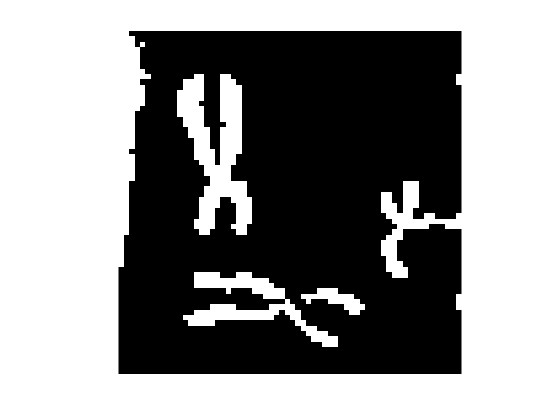
\includegraphics[width=6cm]{fig8a.jpg}
			\subcaption{Image 1}
			\label{fig8a}
		\end{minipage}
		\begin{minipage}[t]{0.48\textwidth}
			\centering
			
\includegraphics[width=6cm]{fig8b.jpg}
			\subcaption{Image 2}
		\end{minipage}
		\caption{Binarized image}
		\label{fig8}
	\end{figure}
	
	
	The binary image result of OTSU algorithm (Fig.~\ref{fig9a}) still has the following defects: (1) the section of the lower chromosome has a fracture; (2) the noise on the both left and right sides of the image cannot be removed. To improve the threshold quality, we adopt some post-processing.
	
	For the fracture of the chromosome graph, we adopt the morphological operations in Image Processing Toolbox in the lower section of the image. The ‘bridge’ operation is employed to bridge the unconnected pixels, while the ‘fill’ operation is used to fill the isolated internal pixel points. The fracture-repaired section will be put back into the original image (Fig.~\ref{fig9b}).
	
	To remove the noise points on the sides of the image, the region growing operation is adopted. Manually choose four points to push into the stack as the seeds, then process the region growing until all the points is labeled in 0 and 1. Thus, the noise points are removed (Fig.~\ref{fig9c}).
	
	\begin{figure}[htbp]
		\centering
		\begin{minipage}[t]{0.3\textwidth}
			\centering
			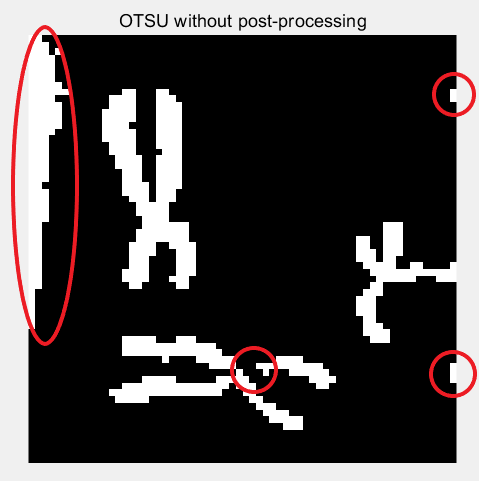
\includegraphics[width=4cm]{without post-processing.png}
			\subcaption{Without post-processing}
			\label{fig9a}
		\end{minipage}
		\begin{minipage}[t]{0.3\textwidth}
			\centering
			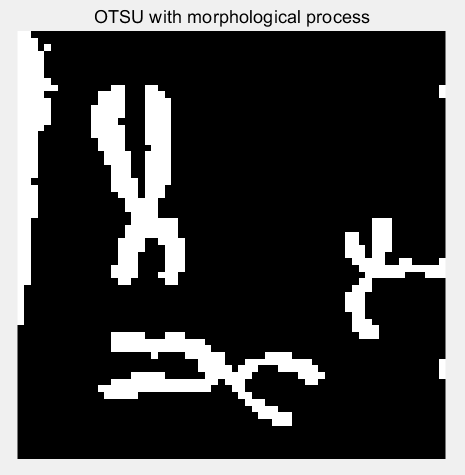
\includegraphics[width=4cm]{morphological process.png}
			\subcaption{After morphological processing}
			\label{fig9b}
		\end{minipage}
		\begin{minipage}[t]{0.3\textwidth}
			\centering
			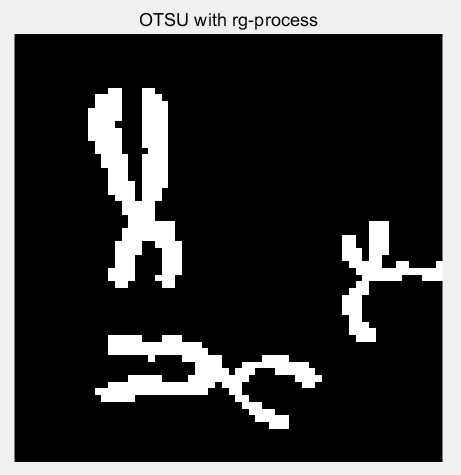
\includegraphics[width=4cm]{rg-process.png}
			\subcaption{After region growing processing}
			\label{fig9c}
		\end{minipage}
		\caption{Post-processing for binarized image 1}
		\label{fig9}
	\end{figure}
	
	
	
	\section{Image Thinning}
	
	\hspace{1.0em}
	Image Thinning generally refers to an operation of Image Skeletonization of binary images. Thinning is the abbreviation of the process of reducing the foreground region of an image from multi-pixel width to unit pixel width. The process largely preserves the extent and connectivity of the original region while throwing away most of the original foreground pixels, which is also one of the main difficulties in algorism design. 
	
	Thinning provides a compact yet effective representation of key topologic and geometric features in an object. The compactness feature of skeletons facilitates efficient assessment of local structural metrics including scale, orientation, topology, geometry, etc.
	
	\subsection{Hilditch thinning algorithm}
	
	\hspace{1.0em}
	The basic principle of the Hilditch algorithm is to determine whether a point in the image is a boundary point or a connected point, and if it is a boundary point, the point can be removed. The whole process is to iterate over each pixel of an image from the top left corner to the bottom right corner, and each iteration removes the outermost layer of pixels from the image, leaving a line in the middle after the layers are peeled off to get the final refined image, i.e., the skeleton line.
	
	The 8 neighbours of $P$ is shown as Fig.~\ref{fig10}. Then the determination of whether a point $P$ should be deleted in an iterative operation is based on whether it satisfies the following six conditions:
	
	\begin{figure}[htbp]
		\centering
		\centering
		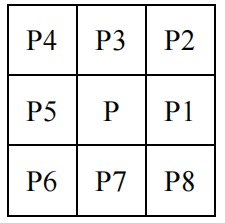
\includegraphics[width=2cm]{Hilditch.png}
		\caption{The 8 neighbors of point $P$ in Hilditch algorithm}
		\label{fig10}
	\end{figure}
	
	\begin{itemize}
		\item $P$ is a foreground pixel.
		\item $P1$, $P3$, $P5$ and $P7$ are not all foreground pixels, i.e., $P$ is a boundary point.
		\item There are at least two foreground pixels in $P1\sim P8$, indicating that $P$ is not an endpoint or isolated point. Endpoints and isolated points cannot be deleted.
		\item The connections parameter of the eight connected regions of $P$ is 1, which ensures that the refinement of the skeleton line will not be broken.
		\item If $P3$ is marked for deletion and $P3$ is 0, the number of linked connections of $P$ is 1, ensuring that the two pixel-wide horizontal bars will not be eroded away.
		\item If $P5$ is marked for deletion and $P5$ is 0, the number of linked connections of $P$ is 1, ensuring that the two pixel-wide vertical bars will not be corroded off.
	\end{itemize}
	
	where the connections parameter of the eight connected regions of $P$ can be calculated as following equation.
	
	\begin{equation}
	\begin{split}
	\begin{aligned}
	N_{c}^{8}(P)=\sum_{i=1}^{4}(\bar{P}_{2i-1}-\bar{P}_{2i-1}\bar{P}_{2i}\bar{P}_{2i+1})
	\end{aligned}
	\end{split}
	\label{eq10}
	\end{equation}
	
	\subsection{Zhang-Suen thinning algorithm}
	
	\hspace{1.0em}
	Zhang-Suen thinning algorithm is an iterative algorithm, and the whole iterative process is divided into the following two steps. The sketch map for the 8 neighbors around point $P1$ is shown in Fig.~\ref{fig11}.
	
	\begin{figure}[htbp]
		\centering
		\centering
		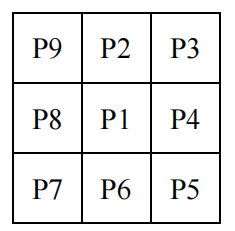
\includegraphics[width=2cm]{Zhang-Suen.png}
		\caption{The 8 neighbors of point $P1$ in Zhang-Suen algorithm}
		\label{fig11}
	\end{figure}
	
	\begin{itemize}
		\item[Step 1.] Loop through all non-zero pixels points and mark as deleted those that meet the following conditions:
			\item The number of foreground pixels in the eight connected region of $P1$ is 2-6.
			\item Cumulative number of occurrences of 0 to 1 in one lap of $P2 \sim P9 \sim P2$ is 1.
			\item $P2\ast P4\ast P6=0$
			\item $P4\ast P6\ast P8=0$
		\item[Step 2.] Loop through all non-zero pixels points and mark as deleted those that meet the following conditions:
			\item The number of foreground pixels in the eight connected region of $P1$ is 2-6.
			\item Cumulative number of occurrences of 0 to 1 in one lap of $P2 \sim P9 \sim P2$ is 1.
			\item $P2\ast P4\ast P8=0$
			\item $P2\ast P6\ast P8=0$
	\end{itemize}

	Loop the above two steps until no pixel is marked for deletion in both steps, and the output is the refined skeleton of the binary image.
	
	\subsection{Rosenfeld thinning algorism}
	
	\hspace{1.0em}
	To explain the Rosenfeld thinning algorism, the following concepts are necessary to be introduced.
	
	\begin{itemize}
		\item Azimuthal boundary point
		
		 For the current pixel P1:
		 \begin{itemize}
			\item If P2 = 0, P1 is the northern boundary point;
			\item If P6 = 0, P1 is the southern boundary point;
			\item If P8 = 0, P1 is the western boundary point;
			\item If P4 = 0, P1 is the eastern boundary point. 
		\end{itemize}
	
		\item Isolated point
		\begin{itemize}
			\item If the value of all 8 connected pixels of P1 is 0, P1 is an isolated point.
		\end{itemize}
	
		\item Endpoint
		\begin{itemize}
			\item If there is one and only one pixel of the 8 connected pixels of P1 has the value of 1, P1 is an endpoint.
		\end{itemize}
		
		\item 8-simple
		\begin{itemize}
			\item If setting the value of P1 to 0 does not change the 8 connectivity of the 8 surrounding pixels, P1 is said to be 8-simple.
		\end{itemize}
		
	\end{itemize}

	Rosenfold algorithm is an iterative algorithm, the operations performed in one iteration are as follows.
	
	\begin{itemize}
		\item[Step 1.] Scan all pixels and delete if the pixel is a northern boundary point and is 8simple but not an isolated point and endpoint.
		\item[Step 2.] Scan all pixels and delete if the pixel is a southern boundary point and is 8simple but not an isolated point and endpoint.
		\item[Step 3.] Scan all pixels and delete if the pixel is an eastern boundary point and is 8simple but not an isolated point and endpoint.
		\item[Step 4.] Scan all pixels and delete if the pixel is a northern boundary point and is 8simple but not an isolated point and endpoint.
	\end{itemize}

	After executing the above 4 steps, an iteration is completed. Repeat the above process until there are no more pixel points in the image that can be deleted, then exit the loop.
	
	\subsection{Look up table Algorithm}
	
	\hspace{1.0em}
	For each current point $P$, there are 256 combinations of values for its surrounding connected eight pixels. If a table with the values of $P$ under these 256 cases was made, whether to delete each point or not can be decided by looking up the table.
	
	The bases for the tabulation process are:
	
	\begin{itemize}
		\item Internal points should not be deleted.
		\item Isolated points should not be deleted.
		\item Endpoints should not be deleted.
		\item For a boundary point $P$, if the connected component does not increase after removing $P$, then $P$ can be deleted.
	\end{itemize}

	According to these bases, a table shown in Fig.~\ref{fig12} was generated.
	
	\begin{figure}[htbp]
		\centering
		\centering
		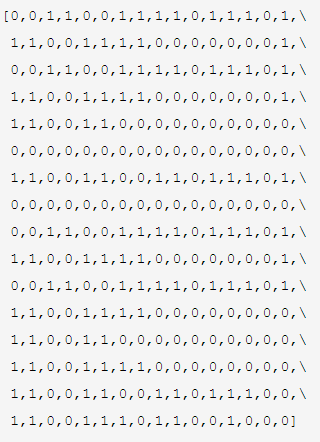
\includegraphics[width=4cm]{table.png}
		\caption{Table for image thinning}
		\label{fig12}
	\end{figure}
	
	The index of the P point in the table can be generated by assigning different values to the surrounding eight points. The assignment factors for the different positions are shown in Fig~\ref{fig13}. The final index of the P is the sum of the surrounding eight pixels’ values multiplied by the assignment factor.
	
	\begin{figure}[htbp]
		\centering
		\centering
		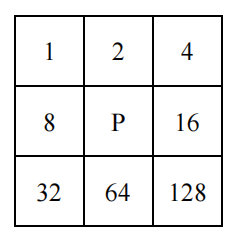
\includegraphics[width=2cm]{Look up table.png}
		\caption{Assignment factors for different positions around $P$}
		\label{fig13}
	\end{figure}
	
	Each iteration will iterate through all the foreground pixels, calculate the index, and look up the table to decide whether the point is deleted or not. The iteration is stopped when no more new points are deleted.
	
	\subsection{Comparison and discussion}
	
	\hspace{1.0em}
	We implemented the above four iterative refinement algorithms and obtained the results as shown in the Fig.~\ref{fig14}. The Helditch algorithm generally performs well, but the final skeleton is slightly distorted compared to the chromosome shape in the original image. The Zhang Suen algorithm can also accomplish the task of thinning, but the quality of the final skeleton is not very good and has more deformation. The Rosenfeld algorithm performs the best, the object is thinned to 1 pixel image and there is no breakage. The skeleton shape maintains the object form in the original picture. Although the Look up Table algorithm has the advantage of fast speed, but it cannot thin the object well, and there are a lot of fracture defects that make the skeletal form not well preserved. So finally, we choose Rosenfeld algorithm to process image thinning.

	\begin{figure}[h]
		\centering
		\begin{minipage}[t]{0.48\textwidth}
			\centering
			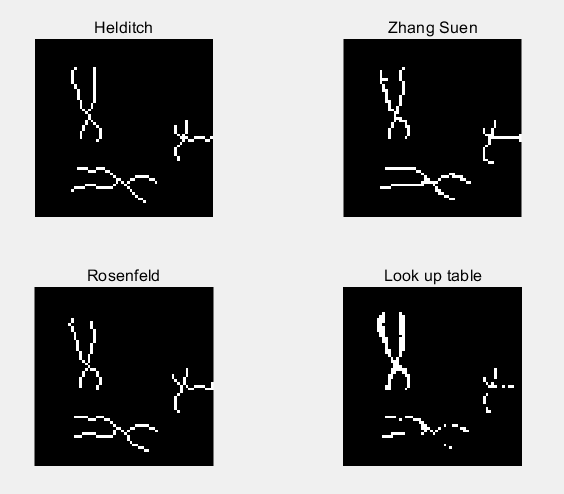
\includegraphics[width=6cm]{result.png}
			\subcaption{Image 1}
		\end{minipage}
		\begin{minipage}[t]{0.48\textwidth}
			\centering
			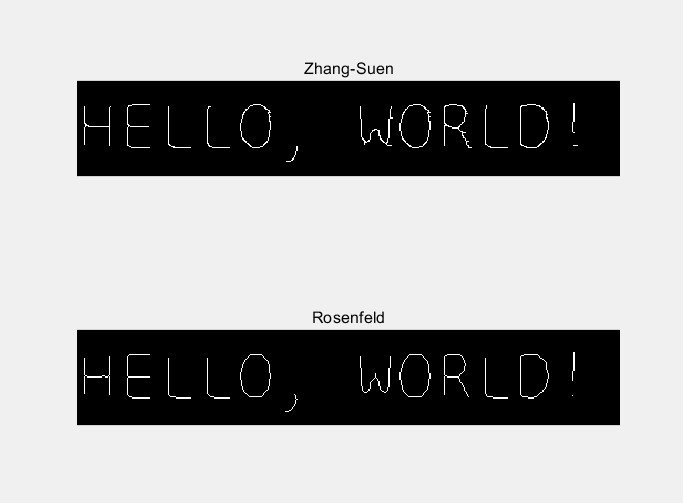
\includegraphics[width=7cm]{thinning result Q2.png}
			\subcaption{Image 2}
		\end{minipage}
		\caption{Comparison results of different thinning algorithm}
		\label{fig14}
	\end{figure}
	
	\subsection{Chosen algorithm}
	
	\hspace{1.0em}
	Finally Rosenfeld method is chosen as the thinning algorithm. The flow of implemented algorithm is shown as below.

	\begin{algorithm}
		%\textsl{}\setstretch{1.8}
		\renewcommand{\algorithmicrequire}{\textbf{Input:}}
		\renewcommand{\algorithmicensure}{\textbf{Output:}}
		\caption{Rosenfeld Algorithm}
		\label{alg2}
		\begin{algorithmic}[1]
			\REQUIRE A binary image
			\ENSURE A binary image showing the skeleton of the objects
			\REPEAT
			\IF {the pixel is an azimuthal boundary point}
			\IF {the pixel is 8-simple}
			\IF {the pixel is not isolate point or endpoint}
			\STATE set the pixel value to 0
			\ENDIF 
			\ENDIF
			\ENDIF
			\UNTIL no longer a pixel deleted
		\end{algorithmic}  
	\end{algorithm}
	
	
	
	\section{Edge detection}
	
	\hspace{1.0em}
	Edge is one of the most basic features of an image and it is generally used when distinguishing the object and the background. Edge could be defined as a discontinuity in the local characteristics of an image. The idea underlying most edge-detection techniques is the computation of a local derivative operator.
	
	We could define a gradient operator where the gradient is a vector pointing in the direction of the most dramatic change in the grey level of the image.
	
	\begin{equation}
	\begin{split}
	\begin{aligned}
	\triangledown \vec{f}=\begin{pmatrix}
	G_{x}\\ 
	G_{y}
	\end{pmatrix}=
	\begin{pmatrix}
	\frac{\partial f}{\partial x}\\ 
	\frac{\partial f}{\partial y}
	\end{pmatrix}
	\end{aligned}
	\end{split}
	\label{eq11}
	\end{equation}
	
	The magnificent is $\triangledown f=mag(\triangledown \vec{f})=(G_{x}^{2}+G_{y}^{2})^{1/2}$, and the gradient is commonly approximated by the absolute values
	
	\begin{equation}
	\begin{split}
	\begin{aligned}
	\triangledown f=\mid G_{x}\mid + \mid G_{y}\mid
	\end{aligned}
	\end{split}
	\label{eq12}
	\end{equation}
	
	Direction of $\triangledown \vec{f}$ at $(x,y)$ is 
	
	\begin{equation}
	\begin{split}
	\begin{aligned}
	\alpha (x,y)=tan^{-1}(G_{x}, G_{y})^{T}
	\end{aligned}
	\end{split}
	\label{eq13}
	\end{equation}
	
	Image edge detection is based on the gradient of an image, and obtaining the gradient of an image translates into using various operators to convolve the image. Therefore core of the image edge detection algorithm therefore lies in the different operators. 
	
	
	
	\subsection{Roberts operator}
	
	\hspace{1.0em}
	The Roberts operator, also known as the cross-difference algorithm, is a gradient algorithm based on cross-differencing, where edge lines are detected by local differencing calculations. It is often used to process low noise images with steep edges and is more effective when the image edges are close to plus 45 degrees or minus 45 degrees.
	
	The mask of roberts operator in the two directions are:
	
	\begin{equation}
	\begin{split}
	\begin{aligned}
	G_{x}=\begin{pmatrix}
	-1 &0 \\ 
	0 &1 
	\end{pmatrix}, \ \ G_{y}=\begin{pmatrix}
	0 &-1 \\ 
	1 &0 
	\end{pmatrix}
	\end{aligned}
	\end{split}
	\label{eq14}
	\end{equation}
	
	To convert it into the form of the formula:
	
	\begin{equation}
	\begin{split}
	\begin{aligned}
	G_{x}=f(i,j)-f(i-1,j-1), \ \ G_{y}=f(i-1,j)-f(i,j-1)
	\end{aligned}
	\end{split}
	\label{eq15}
	\end{equation}
	
	The formula shows that the roberts operator enhances image edges at plus or minus 45 degrees very well. However, the disadvantage is that the positioning of the edges is not very accurate and the extracted edge lines are thick.
	
	\subsection{Prewitt operator}
	
	\hspace{1.0em}
	Prewitt operator is another method which uses the difference in grey scale between the upper and lower, left and right neighbors of a pixel is used to detect edges at their extremes and to remove some of the pseudo-edges, which has a smoothing effect on noise. The principle is to use two directional masks in image space to convolve with the image in the neighborhood, one to detect horizontal edges and one to detect vertical edges.
	
	\begin{equation}
	\begin{aligned}
	G_{x}=\begin{pmatrix}
	-1 &0  &1 \\ 
	-1 &0  &1 \\ 
	-1 &0  &1 
	\end{pmatrix}, \ \ G_{y}=\begin{pmatrix}
	1 &1  &1 \\ 
	0 &0  &0 \\ 
	-1 &-1  &1 
	\end{pmatrix}
	\end{aligned}
	\label{eq16}
	\end{equation}
	
	Compared with the Roberts operator which uses a 2x2 filtering operator, the Prewitt operator uses a 3x3 operator to compute pixel values in specific regions of the image, which results in the edge detection profile of the Prewitt operator being more pronounced in both the horizontal and vertical parts of the image than the edges detected by the Robert operator. After calculating the value of gradient , we need to set a threshold which is used to distinguish the edge according to the relationship between  and the value of threshold.
	
	\subsection{Sobel operator}
	
	\hspace{1.0em}
	The Sobel operator adds the concept of weighting to the Prewitt operator, considering that the distance between neighboring points has a different impact on the current pixel, with the closer the pixel the greater the impact on the current pixel, thus sharpening the image and highlighting the edge contours. The Sobel operator combines Gaussian blurring and differentiation and calculates an approximation of the degree of lightness or darkness of the image, by comparing the degree of lightness or darkness at the edges of the image and recording the specific pixel points in the region above a threshold as edge points. The two directional masks used in sobel operator are:
	
	\begin{equation}
	\begin{aligned}
	G_{x}=\begin{pmatrix}
	-1 &0  &1 \\ 
	-2 &0  &2 \\ 
	-1 &0  &1 
	\end{pmatrix}, \ \ G_{y}=\begin{pmatrix}
	1 &2  &1 \\ 
	0 &0  &0 \\ 
	-1 &-2  &1 
	\end{pmatrix}
	\end{aligned}
	\label{eq17}
	\end{equation}
	
	Because the Sobel operator combines Gaussian smoothing and differential derivatives, the results will be more noise immune and the Sobel operator is a more commonly used method for edge detection when accuracy is not very important.
	
	\subsection{Laplacian operator}
	
	\hspace{1.0em}
	The Laplacian operator is an isotropic second order differential operator with rotational invariance. 
	The formula of second order difference is:
	
	\begin{equation}
	\begin{aligned}
	\triangledown^{2} f= \frac{\partial^{2} f}{\partial x^{2}}+\frac{\partial^{2} f}{\partial y^{2}}
	\end{aligned}
	\label{eq18}
	\end{equation}
	
	The expression could be convert to the discrete form which is suitable for image processing:
	
	\begin{equation}
	\begin{aligned}
	\triangledown^{2} f=f[f(x+1,y)+f(x-1,y)+f(x,y+1)-f(x,y-1)]-4f(x,y)
	\end{aligned}
	\label{eq19}
	\end{equation}
	
	The main idea of Laplacian operator is to find the relationship between the grayscale of the central pixel and the other pixels in the neighborhood by calculating the gradient of the central pixel of the neighborhood in four direction or eight direction and then sum up the gradients. If the central pixel has a higher grey level, the grey level of the central pixel is raised; if not, the grey level of the central pixel is lowered, thus sharpening the image. The mask we used is to calculate the gradient of 8 directions. The mask is:
	
	\begin{equation}
	\begin{aligned}
	G=\begin{pmatrix}
	-1 &-1  &-1 \\ 
	-1 &8  &-1 \\ 
	-1 &-1  &-1 
	\end{pmatrix}
	\end{aligned}
	\label{eq20}
	\end{equation}
	
	When the pixel itself and its neighbors have the same grey value, the result of the Laplacian operator is zero; when the pixel itself has a higher grey value than the mean grey value of its neighbors, the result of the operation is positive; otherwise, it is negative. The edge of the image can therefore be determined by the excess of zero between the positive and negative peaks.
	
	\subsection{Canny operator}
	
	\hspace{1.0em}
	The Canny operator is a multi-stage edge detection operator that combines filtering, enhancement and detection, with the goal of finding an optimal edge profile. The Canny consists of four steps.
	
	\begin{itemize}
		\item[Step 1.]  Smoothing of the image with a Gaussian filter.
	\end{itemize}
	
	The derivative calculation is very sensitive to noise so it is essential to use gaussian filter to smooth the input to avoid enlarging the noise. The method is to multiply each pixel point and its neighborhood by a Gaussian matrix and take the average with weights as the final grey value.
	
	\begin{itemize}
		\item[Step 2.]  Computation of the value and direction of the gradient using a difference with first-order partial derivatives.
	\end{itemize}
	
	Because an edge is a collection of pixels with a large variation in grey value so this step will calculate the value and direction according to Eq.~\ref{eq12} and Eq.~\ref{eq13}.
	
	\begin{itemize}
		\item[Step 3.]  Non-maximal suppression of the gradient amplitude.
	\end{itemize}

	The gradient image obtained from step 2 suffers from uneven edge width, blurring and misidentification so the non-maximal value points of the gradient image need to be suppressed to remove those non-edge pixels. The non-maximum suppression method is used to find the local maxima of the gradient image as edge points and to set the grey scale value of the non-maximum points to 0.
	
	The neighbor around specific pixel could be divided into 4 areas according to the direction as shown in Fig.~\ref{fig15}. The process could be achieved by comparing each pixel with two neighbor pixels that have the same gradient. If the gradient value is not the maximum of the three pixels, the pixel is suppressed, i.e. the pixel is made zero.
	
	\begin{figure}[h]
		\centering
			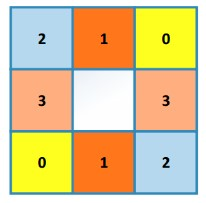
\includegraphics[width=2cm]{fig15.jpg}
		\caption{The four areas divided according to direction}
		\label{fig15}
	\end{figure}
	
	\begin{itemize}
		\item[Step 4.]  Detect and connect the edges using a double thresholding algorithm.
	\end{itemize}

	The edge image obtained in step 3 still has many pseudo-edges, so the Canny algorithm uses a double-thresholding algorithm to detect and connect the edges. If the gradient amplitude at a pixel position exceeds a high threshold, it is retained as an edge pixel and if it is less than the low threshold, it is excluded. If in between, determine if there are pixels in the 8 neighborhood space of the pixel that are above the high threshold, and if so, retain the pixel.
	
	\subsection{Comparison and discussion}
	
	\hspace{1.0em}
	The Roberts operator is the more basic edge detection operator and it is not very accurate. It is suitable  for images with steep edges and little noise, especially for images with many plus or minus 45 degrees edges.
	
	The edge detection results of the Prewitt operator are more pronounced than those of the Roberts operator in both the horizontal and vertical directions. Although the Prewitt operator suppresses noise by averaging the grey values around the pixel, this type of noise suppression is only equivalent to a low-pass filtering operation on the image, which will result in the Prewitt operator being less accurate than the Roberts operator in locating the edges of the image. 
	
	The Sobel operator provides a high level of noise immunity to edge detection by combining Gaussian blurring and first order differential. However, the disadvantage of this algorithm is that it does not strictly separate the subject from the background of the image, which can lead to blurred edge contours. 
	
	The Laplacian operator has a good overall effect, but the operator is very sensitive to noise and it strengthens the noise component, both of which make the operator prone to losing part of the edge orientation information, resulting in some discontinuous detected edges, while the noise immunity is relatively poor.
	
	The canny operator is considered to be the optimal algorithm for edge detection and is much more accurate in identifying image edges than other edge detection algorithms. Even though the effect of our experiment is not quite excellent, the effect of MATLAB built-in canny function works well. The effect for image 1 using different operators are shown in Fig.~\ref{fig16a}.
	
	\begin{figure}[h]
		\centering
		\begin{minipage}[t]{0.35\textwidth}
			\centering
			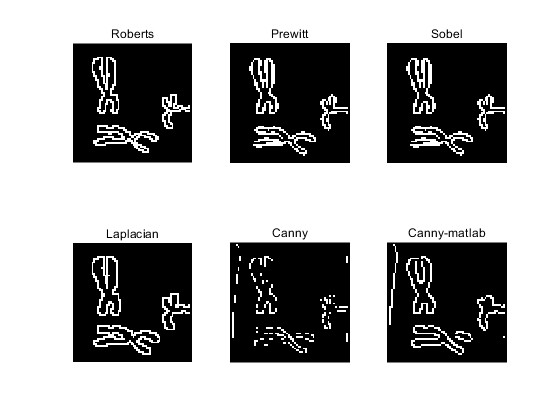
\includegraphics[width=6cm]{fig16a.jpg}
			\subcaption{Effect of different operators for image 1}
			\label{fig16a}
		\end{minipage}
		\begin{minipage}[t]{0.48\textwidth}
			\centering
			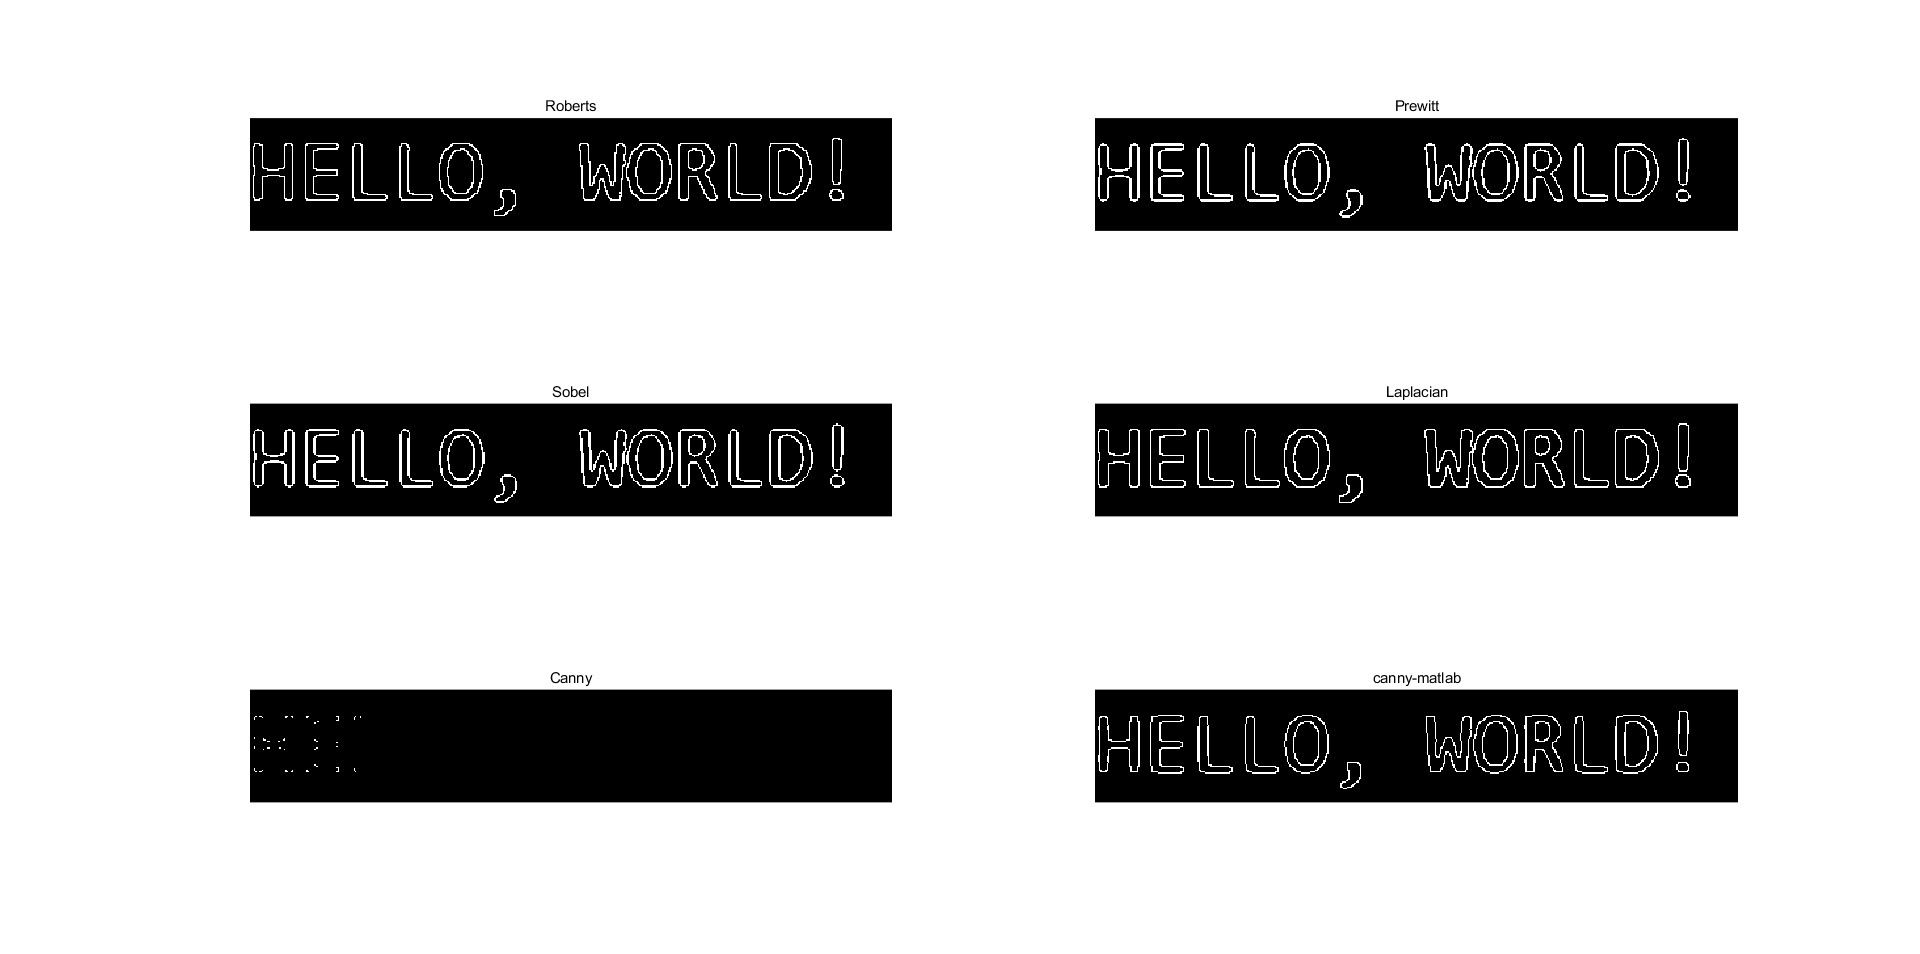
\includegraphics[width=9cm]{fig16b.jpg}
			\subcaption{Effect of different operators for image 2}
			\label{fig16b}
		\end{minipage}
		\caption{Comparison of different edge detection algorithms}
		\label{fig16}
	\end{figure}
	
	
%	\begin{figure}[h]
%		\centering
%		\includegraphics[width=8cm]{fig16.jpg}
%		\caption{The effect of different operators for image 1}
%		\label{fig16}
%	\end{figure}
%	
%	Discription for image 2
%	
%	\begin{figure}[h]
%		\centering
%		\includegraphics[width=12cm]{fig17.jpg}
%		\caption{The effect of different operators for image 2}
%		\label{fig17}
%	\end{figure}

	
	\subsection{Chosen algorithm}
	
	\hspace{1.0em}
	Chosen reason
	
	\begin{algorithm}
		%\textsl{}\setstretch{1.8}
		\renewcommand{\algorithmicrequire}{\textbf{Input:}}
		\renewcommand{\algorithmicensure}{\textbf{Output:}}
		\caption{Laplacian operator}
		\label{alg3}
		\begin{algorithmic}[1]
			\REQUIRE A binary image
			\ENSURE A image with only object's edge 
			\FOR{all central pixels}
				\STATE Multiplying matrix $A$ (central pixel and its neighbors) and matrix $G$ (8 neighbor operator)
				\STATE Sum the gradient value
				\IF{$value>laplaceThreshold$}
					\STATE pixel=1
				\ELSE
					\STATE pixel=0
				\ENDIF
			\ENDFOR
		\end{algorithmic}  
	\end{algorithm}
	
	\section{Labling and segmentation}
	
	\hspace{1.0em}
	The connected components labelling operation performs the unit change from pixel to region of segment. All the pixels belong to the same connected component should be given the same identifying label. Based on this, regional features can be obtained and different objects in the picture can be separated, following with regional operations and decision making.
	
	\subsection{Classical label propagation algorithm}
	
	\hspace{1.0em}
	The basic principle to determine whether two foreground pixels $P_{0}$ and $P_{n}$ belong to the same component is that: if there is a sequence of foreground pixels ($P_{0},P_{1},...,P_{n}$), and $P_{i}$ is a neighbor of $P_{i-1}$ for $i=1,2,…,n$, then $P_{0}$ and $P_{n}$ belong to the same component. 
	
	The classical label propagation makes only one pass through the image. In the ergodic procedure, the image is scanned in rows left to right, top to down. For foreground point $P$ and its 8 connected neighbors shown in Fig.~\ref{fig17}, if $P_{1}$, $P_{2}$, $P_{3}$, $P_{4}$ all have the value of 0, $P$ will be assigned a new label. If one of the points $P_{1}$, $P_{2}$, $P_{3}$, $P_{4}$ is not 0 points, $P$ will be assigned the same label as the non-zero point. If the number of non-zero points among $P_{1}$, $P_{2}$, $P_{3}$, $P_{4}$ is more than 1, $P$ will be assigned the minimum label and an equivalence found will be entered in an equivalence table. Each entry in the equivalence table consists of an ordered pair, whose values are the label numbers.
	
	\begin{figure}[h]
		\centering
		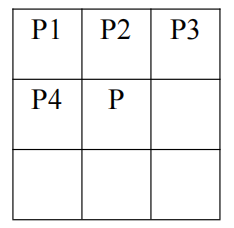
\includegraphics[width=2cm]{classical neighbour.png}
		\caption{$P$ and its neighbors in classical label propagation algorithm}
		\label{fig17}
	\end{figure}

	After the scanning, a median label matrix and a global equivalence table will be generated. Based on the equivalence table initial pairs, equivalent classes can be derived by using the graph search method. Each equivalence class is assigned a unique label by the minimum label in the class. Thus, the final label matrix is generated. Using ‘label2rgb’ function to convert the final label matrix into RGB image. Different components will be colored with different colors.
	
	\subsection{Region growing algorithm}
	
	\hspace{1.0em}
	The region growing algorithm is an operation that aggregate pixels or subregions into larger regions according to a predefined criterion, which is often used for image segmentation. The regions after segmentation need to meet the following conditions: 
	
	\begin{itemize}
		\item $\cup (R_{i}=R)$
		\item $R_{i}$ is a connected region, $i=1,2,...,n$
		\item $R_{i} \cap R_{j}=\o $, for $\forall i,j(i\neq j)$
		\item $H(R_{i})=True$, $i=1,2,...,n$
		\item $H(R_{i} \cup R_{j})=False$, for $\forall i,j(i\neq j)$
	\end{itemize}

	The specific steps of the region growing algorithm are as follows.
	
	\begin{itemize}
		\item[Step1. ] Traversing the image by row, when a foreground point P is encountered, pushing the current point into the stack as the seed point.
		\item[Step2. ] Determine whether the stack is empty. If the stack is non-empty, assign the label to the top element of the stack and pop the top element of the stack. Then push the foreground point of 8 connected neighbors of the top element into the stack.
		\item[Step3. ] Repeat Step 2 until the stack is empty.
		\item[Step4. ] Continue traversing the image by row until the next foreground point is encountered, assigning a new label to the pixel. Then repeat steps 2 - 3 until the image is traversed.
		\item[Step5. ] Using ‘label2rgb’ function to convert the final label matrix into RGB image. Different components will be colored with different colors.
		
	\end{itemize}
	
	\subsection{Comparison and discussion}
	
	\hspace{1.0em}
	As shown in Fig.~\ref{fig18}, both methods can complete the labelling operation very well, and the segmentation quality is about the same. However, the region growing algorithm is significantly faster than the classical label propagation algorithm. It takes 0.164s to complete the labelling using the classical label propagation algorithm, while the region growing algorithm takes only 0.03s. So, we choose the region growing algorithm.
	
	\begin{figure}[h]
		\centering
		\begin{minipage}[t]{0.48\textwidth}
			\centering
			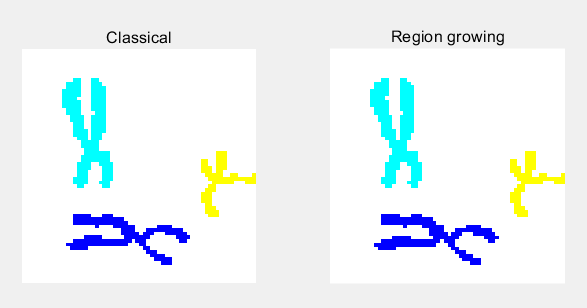
\includegraphics[width=6cm]{label result 1.png}
			\subcaption{Result comparison of labelling operation for image 1}
			\label{fig18a}
		\end{minipage}
		\begin{minipage}[t]{0.48\textwidth}
			\centering
			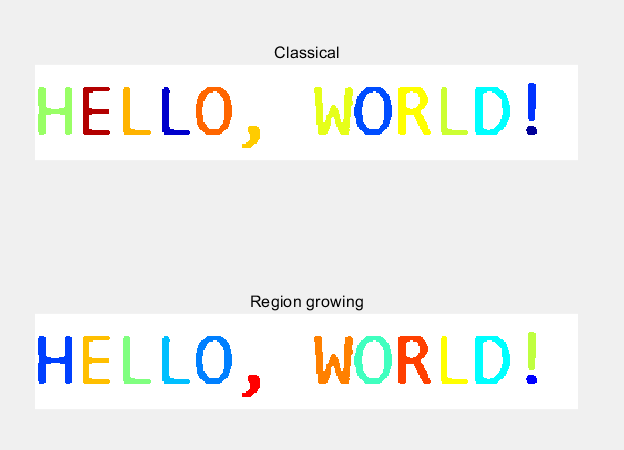
\includegraphics[width=6cm]{label result 2.png}
			\subcaption{Result comparison of labelling operation for image 2}
			\label{fig18b}
		\end{minipage}
		\caption{Comparison of different label algorithms}
		\label{fig18}
	\end{figure}
	
	\subsection{Chosen algorithm}
	
	\hspace{1.0em}
	The finally chosen region growing algorithm is shown below.
	
	\begin{algorithm}
		%\textsl{}\setstretch{1.8}
		\renewcommand{\algorithmicrequire}{\textbf{Input:}}
		\renewcommand{\algorithmicensure}{\textbf{Output:}}
		\caption{Region Growing Algorithm}
		\label{alg4}
		\begin{algorithmic}[1]
			\REQUIRE A binary image
			\ENSURE A RGB image
			\FOR{each pixel}
			\IF{the pixel is poreground point}
				\STATE Push the point into stack
				\REPEAT	
					\STATE Assign the current label number to the top element and pop it
					\STATE Push the foreground point of the 8 neighbors of the top element into stack
				\UNTIL{the stack is empty}
				\STATE Update label number
			\ENDIF
			\ENDFOR
			\STATE Convert the final label matrix into RGB image
		\end{algorithmic}  
	\end{algorithm}
	
	\subsection{Object seperation}
	
	\hspace{1.0em}
	For image 2, the characters need to be separate. The separate algorithm is designed as follows.
	
	\begin{itemize}
		\item[Step 1. ] For a particular label, find all pixels belong to this component. Calculate the horizontal distance r from each pixel to the leftmost pixel and the vertical distance c from each pixel to the uppermost pixel.
		\item[Step 2. ] Take the segment with length of ($r_{max}+20$) and width of ($c_{max}+20$) to generate the new image of the corresponding label.
		\item[Step 3. ] Repeat the above steps until all labels have the new image.
	\end{itemize}

	The result is shown in Fig.~\ref{fig19}.
	
		\begin{figure}[htbp]
		\centering
		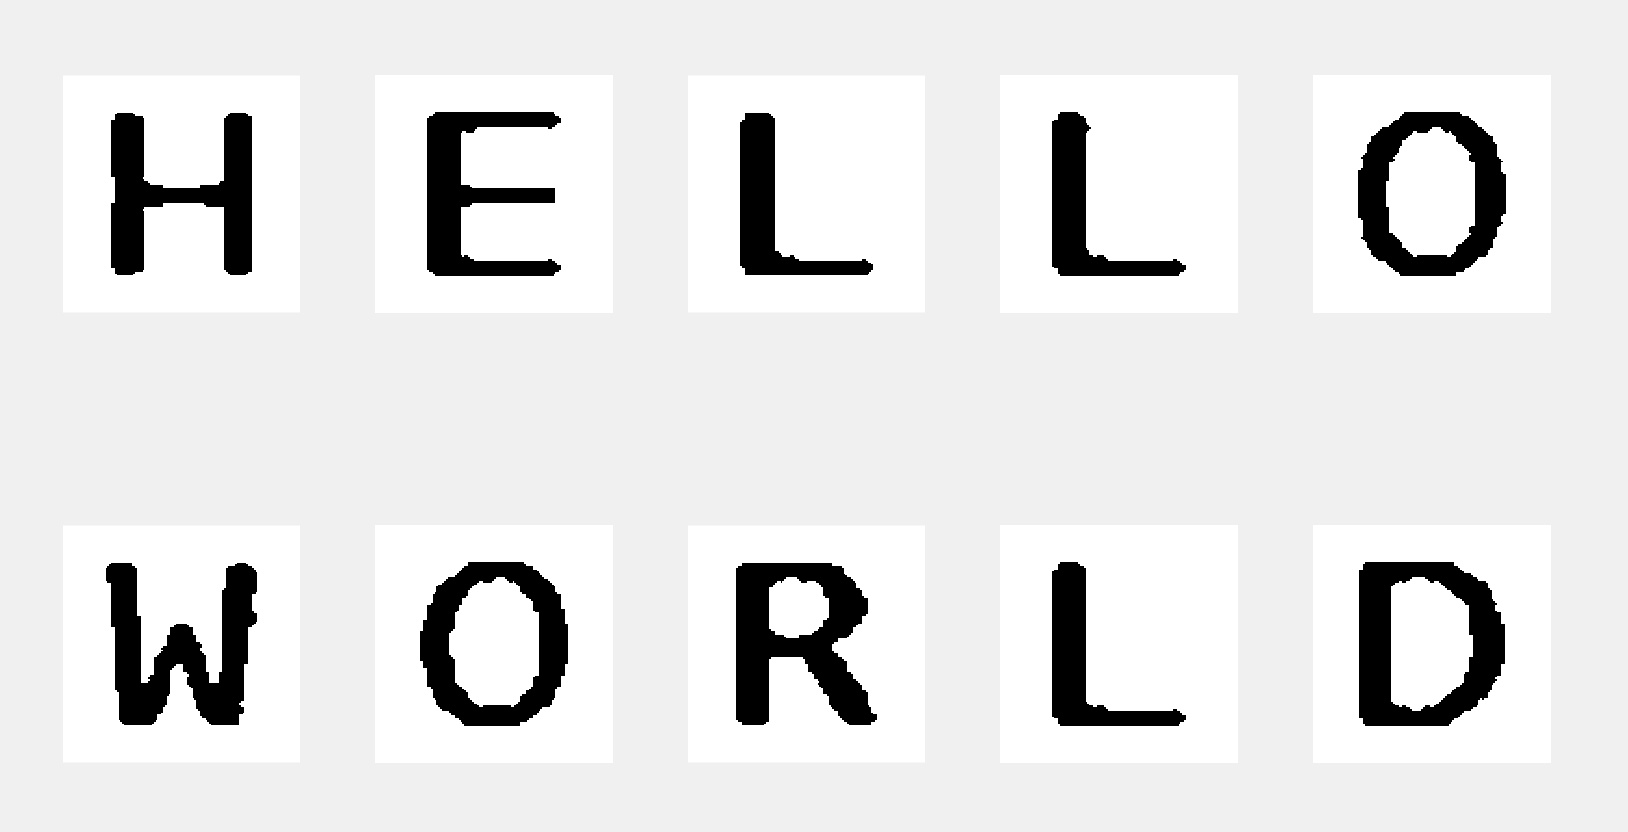
\includegraphics[width=8cm]{result seperate.png}
		\caption{Result of separation for image 2}
		\label{fig19}
	\end{figure}
	
	
	\section{Image rotation}
	
	\hspace{1.0em}
	The kind of image rotation method could be divided into forward mapping and backward mapping. Forward mapping uses the coordinated of original image to calculate the new coordinates of rotated image and the grayscale values are passed through the process. This method could generate regular noise. On the contrary, the backward begins from the rotated image to find the point that corresponds to the original image. We applied these methods respectively in the project.
	
	\subsection{Forward mapping}
	
	\hspace{1.0em}
	The process uses three matrices to rotate image. The first step is to transform the origin of coordinate from the top left corner to the center of the image. Assuming the width and height of image is $h$ and $h$, the coordinate of a pixel is $(x_{0},y_{0})$ and the transformed point is $(x_{1},y_{1})$, the process is:
	
	\begin{equation}
		\begin{pmatrix}
		x_{1} &y_{1}  &1 
		\end{pmatrix}=\begin{pmatrix}
		x_{0} &y_{0}  &1 
		\end{pmatrix}\begin{pmatrix}
		1 &0  &0 \\ 
		0 &-1  &0 \\ 
		-0.5w &-0.5h  &1 
		\end{pmatrix}
		\label{eq21}
	\end{equation}
	
	The rotation angle is set to $\theta$, the point through rotating is $(x_{2},y_{2})$, the rotation operation is:
	
	\begin{equation}
	\begin{pmatrix}
	x_{2} &y_{2}  &1 
	\end{pmatrix}=\begin{pmatrix}
	x_{1} &y_{1}  &1 
	\end{pmatrix}\begin{pmatrix}
	cos\theta &-sin\theta  &0 \\ 
	sin\theta &cos\theta  &0 \\ 
	0 &0  &1 
	\end{pmatrix}
	\label{eq22}
	\end{equation}
	
	The last step is to inverse the coordinate, the point will be $(x_{3},y_{3})$:
	
	\begin{equation}
	\begin{pmatrix}
	x_{3} &y_{3}  &1 
	\end{pmatrix}=\begin{pmatrix}
	x_{2} &y_{2}  &1 
	\end{pmatrix}\begin{pmatrix}
	1 &0  &0 \\ 
	0 &-1  &0 \\ 
	0.5w &0.5h  &1 
	\end{pmatrix}
	\label{eq23}
	\end{equation}
	
	Because the rotation could convert some value to non-integer, we need to perform rounding operations. The result is shown in Fig.~\ref{fig20}. It is obvious there is regular noises in the image.
	
	\begin{figure}[htbp]
		\centering
		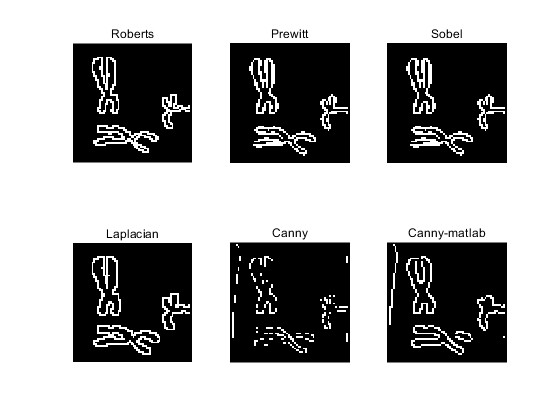
\includegraphics[width=12cm]{fig16a.jpg}
		\caption{The effect of different operators for image 2}
		\label{fig20}
	\end{figure}
	
	\subsection{Backward mapping}
	
	\hspace{1.0em}
	Backward mapping begins with the rotated image, find the point corresponding to the original image and pass the grey scale value from the original image, so that each pixel of the rotated image could correspond to a point in the original image after coordinate transformation and interpolation. Interpolation is a very critical step in this process. We applied the nearest neighbor interpolation and bilinear interpolation.
	
	\subsubsection{Nearest neighbor interpolation}
	
	\hspace{1.0em}
	The main idea for this method is to make the grey value of the transformed pixel equal to the grey value of the nearest input pixel. As shown in Fig.~\ref{fig21}, four $Q$ points are from the original image and according to principle of nearest, the value of $P$ point should equal to $Q3$.
	
	\begin{figure}[htbp]
		\centering
		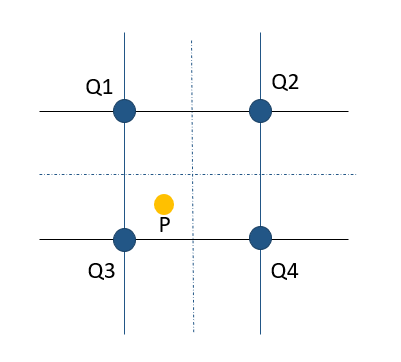
\includegraphics[width=4cm]{nni.png}
		\caption{An example of nearest neighbor interpolation}
		\label{fig21}
	\end{figure}

	This method only use the value of nearest pixel without considering the influence of other neighboring pixels, resulting in a significant discontinuity in gray value and an obvious mosaic.
	
	\subsubsection{Bilinear interpolation}
	
	\hspace{1.0em}
	The main idea for Bilinear interpolation is using linear interpolation in two directions to get a point. As shown in Fig.~\ref{fig22} the first linear interpolation in the $x$ direction to obtain $R1$ and $R2$, and then the second linear interpolation in the $y$ direction gives $P$.
	
	\begin{figure}[htbp]
		\centering
		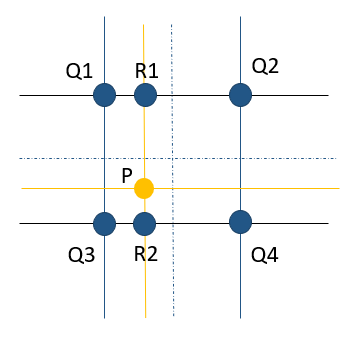
\includegraphics[width=4cm]{bi.png}
		\caption{An example of Bilinear interpolation}
		\label{fig22}
	\end{figure}

	The bilinear interpolation method is better than the nearest neighbor interpolation method but the computation is a bit larger and the program takes a bit longer to run. The bilinear interpolation could generate higher quality images and basically overcomes the discontinuity of the nearest neighbor interpolation grayscale value because it takes into account the correlation effect of the four direct neighbors around the sample point to be measured on the sample point. The results of image rotation using backward mapping is shown in Fig.~\ref{fig23}, the left column uses nearest neighbor interpolation and the right one uses bilinear interpolation.
	
	
	\begin{figure}[htbp]
		\centering
		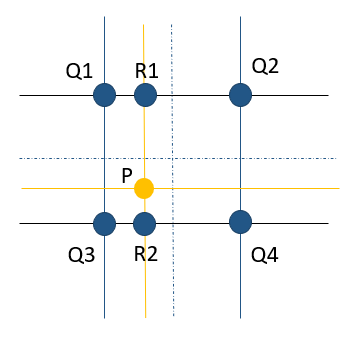
\includegraphics[width=4cm]{bi.png}
		\caption{An example of Bilinear interpolation}
		\label{fig23}
	\end{figure}
	
	
	\section{Classifier design using machine learning methods}
	
	\section{APP design}
	
	\section{Conclusion}
	
	\hspace{1.0em}
	
	
%	\section*{Acknowledgments}
	%MS++++++++++++++++++++++++++++++ Reference ++++++++++++++++++
	%% 参考文献请看下一节详细介绍。
	
	
%	\bibliographystyle{IEEEtran}
%	
%	\bibliography{ref_5405}{}
	
	\newpage
	
%	\begin{appendices}
%		
%		\section{Appendix}
%		
%		
%	\end{appendices}
	
\end{document}